\section{Expressivity}\label{expressivity}

In this section we compare the expressive power of memory logics
with respect to both the modal and hybrid logics.
But comparing the expressive power of these logics poses a complication
because, strictly speaking, each of them uses a different class of models.
We would like to be able to define a natural mapping between models
of each logic, similar to the natural mapping that exists between
Kripke models and first-order models~\cite{BRV01}.

Such a mapping is easy to define in the case of $\cMLRKE$ where the model is interpreted with $S=\emptyset$: each
Kripke model $\diam{W,\rels,V}$ can be identified with the $\cMLRKE$
model $\diam{W,\rels, V, \emptyset}$. Similarly, for formulas
which are sentences, the $\cMLRKE$ model $\diam{W,\rels,V,\emptyset}$ can be identified with the hybrid model
$\diam{W,\rels,V,g}$ (for $g$ arbitrary).
%
Since models for the $\cMLRKE$ logic coincide with those of
$\cMLRKME$, the same applies for the mapping between Kripke models
and $\cMLRKME$ models.
%
As we will discuss below, it is harder to find such a natural way to
transform models for the case of $\cMLRK$ and $\cMLRKM$: the most
natural way seems to involve a shift in the signature of the
language.

\begin{defn}[$\mathcal{L} \le \mathcal{L'}$]
We say that
$\mathcal{L'}$ is \emph{at least as expressive as} $\mathcal{L}$
(notation $\mathcal{L} \le \mathcal{L'}$) if it is possible to
define a function $\Tr$ between formulas of  $\mathcal{L}$ and $\mathcal{L'}$
such that for every model $\model$ and every formula $\varphi$ of $\mathcal{L}$
we have that
\[
\model \models_\mathcal{L} \varphi \mbox{ iff } \model \models_{\mathcal{L}'} \Tr(\varphi).
\]

We say that $\mathcal{L'}$ is \emph{strictly more expressive} than $\mathcal{L}$
(notation $\mathcal{L} < \mathcal{L'}$) if $\mathcal{L} \le \mathcal{L'}$ but
not $\mathcal{L}' \le \mathcal{L}$.  And we say that $\gL$ and $\gL'$ are equally
expressive (notation $\gL = \gL'$) if $\gL \le \gL'$ and $\gL' \le \gL$.
\end{defn}

\begin{figure}
\begin{center}
\begin{tikzpicture}[>=latex]
  \node[draw,rounded corners,minimum height=2.5cm,minimum width=1cm] (b1) at (3,1.25) {};
  \node[draw,rounded corners,minimum height=2.5cm,minimum width=1cm] (b2) at (5,1.25) {};
    \node[draw,rounded corners,minimum height=2.5cm,minimum width=1.4cm] (b3) at (7,1.25) {};

  \node (n0) at (1.2,1.25) {$\mathcal{K}$};
  \node (n3) at (3,2) {$\cMLRKM$};%L3
  \node (n4) at (3,.5) {$\cMLRKME$};%L4
  \node (n1) at (5,2) {$\cMLRK$};%L1
  \node (n2) at (5,.5) {$\cMLRKE$};%L2
  \node (n5) at (7,2) {$\cMLS$};%L5
  \node (n6) at (7,.5) {$\hlogic$};%HL

  \draw [->] (n0) -- (b1);
  \draw [->] (b1) -- (b2);
  \draw [->] (b2) -- (b3);

  \draw [<->,dashed] (n3) edge (n4);
  \draw [<->,dashed] (n1) edge (n2);
  \draw [<->,dashed] (n5) edge (n6);
\end{tikzpicture}
\end{center}
\caption{Expressive power.}\label{fig-expressivity}
\end{figure}

\tb{SS: mejor poner las lineas punteadas como doble flechas
punteadas}



The summary of the results we are going to establish in this section
is shown in Figure~\ref{fig-expressivity}.  In the figure, a full arrow
between two logics $\gL$ and $\gL'$ means that $\gL < \gL'$. Double headed
arrows link languages with the same expressive power.  We use dashed
arrows when a change in the signature is required in the proof, and this is
the first result we are going to show.

\tb{SS: no hay double headed arrows. Entre $\hlogic$ y stack hay
cambio de signatura? Si no hay, deberia ser double headed arrow}

\begin{thm} \
\begin{enumerate}
\item $\cMLRKE$ over the signature $\diam{\prop \cup \{\mathit{known}\}, \rel}$ is equivalent to $\cMLRK$ over the signature $\diam{\prop, \rel}$
\item $\cMLRKME$ over the signature $\diam{\prop \cup \{\mathit{known}\}, \rel}$ is equivalent to $\cMLRKM$ over the signature $\diam{\prop, \rel}$
\end{enumerate}
\end{thm}

\begin{pf}
The argument for item $2$ is exactly the same as the one for item $1$.  Hence let's
prove $\cMLRKE=\cMLRK$ (over the appropriate signatures).

We start by associating every model $\gM=\tup{W,\rels,V,S}$ of $\cMLRK$ over the signature $\diam{\prop, \rel}$ with the model $\gM'=\tup{W,\rels,V',\emptyset}$
of $\cMLRKE$ over the signature $\diam{\prop \cup \{\mathit{known}\}, \rel}$ where $V'$ is identical to $V$ over $\prop$ and $V'(\mathit{known}) =S$.
\smallskip

\noindent $[\cMLRKE \le \cMLRK]$: use the translation $\Tr$ that
only rewrites the propositional symbol $\mathit{known}$ as $\known$
in any formula of $\cMLRKE$. Clearly for any formula $\varphi \in
\cMLRKE$ we have that $\gM',w \models \varphi$ iff $\gM,w \models
\Tr(\varphi)$.
\smallskip

\noindent $[\cMLRK \le \cMLRKE]$: use the translation $\Tr$ that
only rewrites $\known$ as $(\known \vee \mathit{known})$ in any
formula of $\cMLRK$. Clearly for any formula $\varphi \in \cMLRK$ we
have that $\gM,w \models \varphi$  iff $\gM',w \models
\Tr(\varphi)$.
\end{pf}

On the other hand, the freedom to decide when to remember one state
gives $\cMLRK$ and $\cMLRKE$ more expressive power when compared
with $\cMLRKM$ and $\cMLRKME$.


\begin{thm}\label{thm:four-le-two}
$\cMLRKM < \cMLRK$ and $\cMLRKME < \cMLRKE$.
\end{thm}

\begin{pf}
We only prove the result for $\cMLRKM < \cMLRK$ as the other case is
identical.
\smallskip

\noindent
$[\cMLRKM \leq \cMLRK]$: It is easy to see that there is a translation \Tr\ from $\cMLRKM$-
to $\cMLRK$-formulas which maps $\ttup{r}\varphi$ to
$\remember\diam{r}\varphi$ and verifies $\model \models_{\cMLRKM}
\varphi$ iff $\model \models_{\cMLRK} \Tr(\varphi)$.
\smallskip

\noindent
$[\cMLRK \not\leq \cMLRKM]$: Let
$\model_1=\diam{\{w,v,r\}, R_1, V_1, \emptyset}$ and
$\model_2=\diam{\{w,v,r\}, R_2, V_2, \emptyset}$ such that
$R_1=\{(w,v),(v,r),(r,w)\}$, $R_2=\{(w,v),(v,r),(r,v)\}$ and $V_1(p)
= V_2(p) = \emptyset$ for all $p \in \prop$, as shown in Figure~\ref{fig:L3L1}.

\begin{figure}
\begin{center}
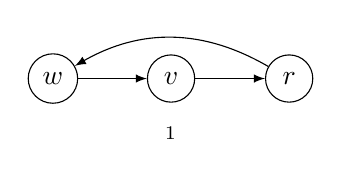
\begin{tikzpicture}[>=latex]
  \node (n1) at (0,0) [shape=circle,draw,minimum height=.6cm] {$w$} ;
  \node (n2) at (1.5,0) [shape=circle,draw,minimum height=.6cm] {$v$} ;
  \node (n3) at (3,0) [shape=circle,draw,minimum height=.6cm] {$r$} ;

  \draw [->] (n1) -- (n2);
  \draw [->] (n2) -- (n3);
  \draw [->] (n3) edge[bend right=30] (n1);

  \node at (1.5,-.7) {$\model_1$};
\end{tikzpicture}
\hspace{1cm}
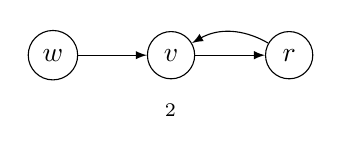
\begin{tikzpicture}[>=latex]
  \node (n1) at (0,0) [shape=circle,draw,minimum height=.6cm] {$w$} ;
  \node (n2) at (1.5,0) [shape=circle,draw,minimum height=.6cm] {$v$} ;
  \node (n3) at (3,0) [shape=circle,draw,minimum height=.6cm] {$r$} ;

  \draw [->] (n1) -- (n2);
  \draw [->] (n2) -- (n3);
  \draw [->] (n3) edge[bend right=30] (n2);

  \node at (1.5,-.7) {$\model_2$};
\end{tikzpicture}
\end{center}
\caption{$\cMLRKE\not=\cMLRKME$.}
\label{fig:L3L1}
\end{figure}

We prove that $\model_1$ and $\model_2$ are $\cMLRKM$-bisimilar. As
every state in both models has a unique successor, Duplicator has
only one way of playing, and this only way is indeed a winning
strategy. From this follows that no formula in $\cMLRKM$ can
distinguish $\model_1$ and $\model_2$. On the other hand, let
$\varphi = \diam{r}\remember\diam{r}\diam{r}\known$ be a
$\cMLRK$-formula. It is easy to see that $\model_1,w \not \models
\varphi$, but $\model_2, w \models \varphi$.
\end{pf}


We will now compare the expressive power of memory logics with
the basic modal logic $\bml$.

\subsection{Memory Logics and Modal Logics}

Because models of $\K$ are different from models for memory logics
we should start by defining how are we going to match them.  In this
case, it seems that we don't have other option but to change the
signature.  But even over a suitable extended signature, $\bml$ is
less expressive than $\cMLRKM$.

It is not difficult to see intuitively that $\remember$ and $\known$ do bring
additional expressive power into the language of $\bml$: with their
help we can detect cycles in a given model, while formulas of $\K$
are invariant under unraveling.

\begin{thm}
$\bml$ over the signature $\diam{\prop \cup \{known\}, \rel}$ is
strictly less expressive than $\cMLRKM$ over the signature
$\diam{\prop, \rel}$.
\end{thm}

\begin{pf}
\tb{modify proof below so that it works with $\cMLRKM$.\\
(diego) tan solo cambie el lenguaje, esta bien la demo asi, no?}

Showing that $\bml\leq\cMLRKM$ is straightforward as $\bml$ is a
sub-language of $\cMLRKM$.  Hence, we can take $\Tr$ to be the
identity function.

To see that $\cMLRKM\not\leq\bml$, let
$\model_1=\diam{\{w\},\{(w,w)\},\emptyset}$ and
$\model_2=\diam{\{u,v\},\{(u,v),(v,u)\},\emptyset}$ be two Kripke
models as shown in Figure~\ref{fig:L3K}. It is known that they are $\bml$ bisimilar
(see~\cite{BRV01}). On the other hand, the equivalent $\cMLRKM$
models are distinguishable by $\varphi=\remember \diam{r}\known$.
%
\begin{figure}
\begin{center}
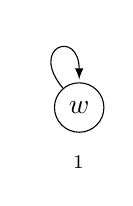
\begin{tikzpicture}[>=latex]
  \node (n1) at (0,0) [shape=circle,draw,minimum height=.6cm] {$w$} edge [in=90, out=130,loop] ();

  \node at (0,-.7) {$\model_1$};
\end{tikzpicture}
\hspace{2cm}
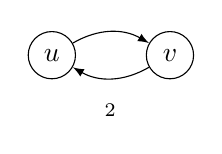
\begin{tikzpicture}[>=latex]
  \node (n2) at (0,0) [shape=circle,draw,minimum height=.6cm] {$u$} ;
  \node (n3) at (1.5,0) [shape=circle,draw,minimum height=.6cm] {$v$} ;

  \draw [->] (n2) edge[bend left=30] (n3);
  \draw [->] (n3) edge[bend left=30] (n2);

  \node at (.75,-.7) {$\model_2$};
\end{tikzpicture}
\end{center}
\caption{$\cMLRKM\not=\bml$.}
\label{fig:L3K}
\end{figure}
%
\end{pf}



\subsection{Memory Logics and Hybrid Logics}

To prove that $\cMLRKE$ is strictly less expressive than $\hlogic$,
we will define a translation that maps formulas of $\tle$ into
sentences of $\hlogic$. Intuitively, it is clear that we can use
$\downarrow$ to simulate $\remember$, but $\known$ does not
distinguishes between different memorized states (while nominals
bound by $\downarrow$ do distinguish them).  We can solve this using
disjunction to gather together all previously remembered states.


%\begin{defn}[Model equivalence]
%We say that a memory logic model $\model_1= \diam{W,\rels,V_1,S}$ over
%$\diam{\prop, \rel}$ is equivalent to a Kripke model over
%$\diam{\prop\cup\{\mathit{known}\}, \rel}$  $\model_2= \diam{W,\rels,V_2}$ if
%$V_1(p) = V_2(p)$ for any $p \not= \mathit{known}$, and $V_2(k) = S$.
%Moreover, we say that $\model_1$ is  equivalent to a $\hlogic$
%model $\model'_2$ over $\diam{\prop\cup\{k\}, \rel,\var}$ when %$\model'_2=\diam{W,\rels,V_2,g}$, for any arbitrary assignment $g$.
%
% To each $\tl$ model $\model_\tl= \diam{W,\{R_i\},V,S}$, we associate
% a Kripke model $\model = \diam{W,\{R_i\},V'}$, where $V(p) = V'(p)$
% for any $p \not= k$, and $V'(k) = S$.
%\end{defn}


\begin{thm}\label{thm:tle_leq_hlogic}
$\cMLRKE\leq\hlogic$.
\end{thm}

\begin{pf}
The translation $\Tr$, taking $\cMLRKE$-formulas over the signature
$\diam{\prop,$ $\rel}$ to $\hlogic$ sentences over the signature
$\diam{\prop, \rel, \nom}$ is defined for any finite set $N
\subseteq \nom$ as follows:
$$
\begin{array}{rcl}
\Tr_N(p) & = & p \quad p \in \prop\\
\Tr_N(\known) & = & \bigvee_{i \in N} i \\
\Tr_N(\lnot \varphi) & = & \lnot \Tr_N(\varphi) \\
\Tr_N(\varphi_1 \land \varphi_2) & = & \Tr_N(\varphi_1) \land \Tr_N(\varphi_2) \\
\Tr_N(\diam{r} \varphi) & = & \diam{r} \Tr_N(\varphi) \\
\Tr_N(\remember \varphi) & = & \down i. \Tr_{N\cup\{i\}}(\varphi)
\quad \textrm{where $i \notin N$.}
\end{array}
$$

\noindent A simple induction shows that $\model, w \models \varphi$
iff $\model, g, w \models \Tr_\emptyset(\varphi)$, for any $g$.
\end{pf}

Finally we arrive to the most interesting question in this section:
as we already mentioned, $\cMLRKE$ seems to be weaker than $\hlogic$
because it allows us to remember that we have already visited a
given state, but we cannot distinguish among different visited
states. Indeed, we can prove that $\cMLRKE$ is strictly less
expressive than $\hlogic$, but the proof is slightly involved.


\begin{thm} \label{thm:tle_not_equal_hlogic}
$\hlogic\not\leq\cMLRKE$.
\end{thm}

\begin{pf}
Let $\model_1=\diam{\omega,R_1,\emptyset,\emptyset}$ and
$\model_2=\diam{\omega,R_2,\emptyset,\emptyset}$, where $R_1=\{(n,m)
\mid n\not= m\} \cup \{(0,0)\}$ and $R_2=\{(n,m) \mid n\not= m\}
\cup \{(0,0),(1,1)\}$ (the models are shown in Figure~\ref{fig}, the
accessibility relation is the non-reflexive transitive closure of the arrows shown
in the picture).

\begin{figure}
\begin{center}
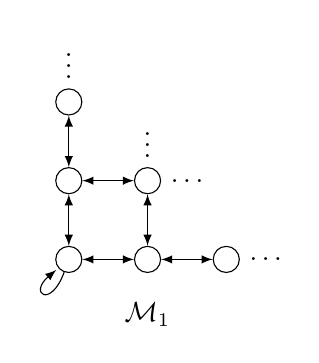
\begin{tikzpicture}[>=latex]

  \node (n11) at (0,0) [shape=circle,draw] {} edge [in=220, out=250,loop] ();
  \node (n22) at (1,1) [shape=circle,draw, label=right:$\dots$, label=above:$\vdots$] {};
  \node (n12) at (0,1) [shape=circle,draw] {} ;
  \node (n21) at (1,0) [shape=circle,draw] {};
  \node (n13) at (0,2) [shape=circle,draw, label=above:$\vdots$] {};
  \node (n31) at (2,0) [shape=circle,draw, label=right:$\dots$] {};

  \draw [<->] (n11) -- (n12);
  \draw [<->] (n21) -- (n22);
  \draw [<->] (n12) -- (n22);
  \draw [<->] (n11) -- (n21);
  \draw [<->] (n21) -- (n31);
  \draw [<->] (n12) -- (n13);

  \node at (1,-.7) {$\mathcal{M}_1$};

\end{tikzpicture}
\hspace{10mm}
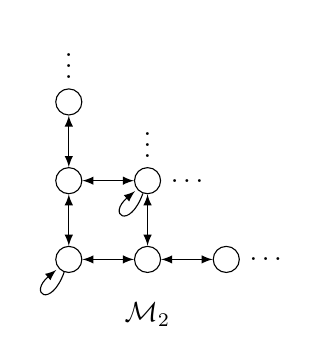
\begin{tikzpicture}[>=latex]

  \node (n11) at (0,0) [shape=circle,draw] {}
                       edge [in=220, out=250,loop] ();
  \node (n22) at (1,1) [shape=circle,draw, label=right:$\dots$, label=above:$\vdots$] {}
                       edge [in=220, out=250,loop] ();
  \node (n12) at (0,1) [shape=circle,draw] {} ;
  \node (n21) at (1,0) [shape=circle,draw] {};
  \node (n13) at (0,2) [shape=circle,draw, label=above:$\vdots$] {};
  \node (n31) at (2,0) [shape=circle,draw, label=right:$\dots$] {};

  \draw [<->] (n11) -- (n12);
  \draw [<->] (n21) -- (n22);
  \draw [<->] (n12) -- (n22);
  \draw [<->] (n11) -- (n21);
  \draw [<->] (n21) -- (n31);
  \draw [<->] (n12) -- (n13);

  \node at (1,-.7) {$\mathcal{M}_2$};
\end{tikzpicture}
\end{center}

%\begin{center}
%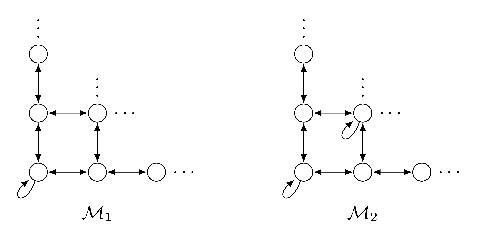
\includegraphics[scale=0.8]{figure1.eps}
%\medskip
\caption{Two $\cMLRKE$-bisimilar models}\label{fig}
\end{figure}

We prove that $\model_1,0\bisim\model_2,0$ showing the winning
strategy for Duplicator. Intuitively, the strategy for Duplicator
consists in the following idea: whenever one player is in
$(\model_1,0)$ the other will be in $(\model_2,0)$ or
$(\model_2,1)$, and conversely whenever a player is in
$(\model_1,n)$, $n>0$ the other will be in $(\model_2,m)$, $m>1$.
This is maintained until Spoiler (if ever) decides to remember a
state. Once this is done, then any strategy will be a winning one
for Duplicator.


Being a bit more formal, the winning strategy will have two stages. While Spoiler does not remember any reflexive
state, Duplicator plays with the following strategy: if Spoiler
chooses $0$ in any model, Duplicator chooses $0$ in the other one;
if Spoiler chooses $n>0$ in $\model_1$, Duplicator plays $n+1$ in
$\model_2$; if Spoiler chooses $n>0$ in $\model_2$, Duplicator plays
$n-1$ in $\model_1$.

Notice that with this strategy Spoiler chooses
a reflexive state if and only if Duplicator answers with a reflexive
one. This is clearly a winning strategy. If ever Spoiler decides to
remember a reflexive state, Duplicator starts using the following
strategy: if Spoiler selects a state $n$, Duplicator answers with an
agreeing state $m$ of the opposite model. Notice that this is always
possible since both $n$ and $m$ see infinitely many non remembered
states and at least one remembered state. Therefore $\model_1,w \bisim \model_2, w$.

On the other hand, let $\varphi$ be the formula $\down i. \diam{r}(i
\land \diam{r}(\lnot i \land \down i.\diam{r}i))$. It is easy to see
that $\model_1, w \not \models \varphi$ but $\model_2, w \models
\varphi$.
\end{pf}

\begin{cor}
$\cMLRKE<\hlogic$.
\end{cor}

\begin{pf}
Straightforward from Theorems~\ref{thm:tle_leq_hlogic}
and~\ref{thm:tle_not_equal_hlogic}.
\end{pf}

The basic idea behind the proof of
Theorem~\ref{thm:tle_not_equal_hlogic} is that if the relations
$R_1$ and $R_2$ extend the set $\{(n,m) \mid n\not= m\}$, then
$\cMLRKE$ can distinguish between irreflexive and non irreflexive
frames, but it cannot distinguish frames with a different number of
reflexive nodes.

There is a number of interesting remarks to be made above the
previous proof. First, notice that it is essential for the winning
strategy of Duplicator that each state in a model is related to
infinitely many others.


We have already shown that $\cMLRKE \not= \hlogic$ and we used a
pair of infinite models to distinguish both logics. We now analyze
the question whether $\cMLRKE \not= \hlogic$ on image-finite models.
We prove that $\hlogic \not \leq \cMLRKE$ on image-finite models
showing that there cannot exist an equivalence preserving
translation for finite models from $\hlogic$ to $\cMLRKE$


\begin{thm}
There is no translation $\Tr$ from $\hlogic$-sentences to
$\cMLRKE$-formulas such that for every finite model $\model$ and
every $\hlogic$-sentence $\varphi$ we have $\model \models
\varphi$ iff $\model \models \Tr(\varphi)$.
\end{thm}
\begin{pf}
Let us suppose that such translation $\Tr$ exists. Let
\[
 \varphi =
\down i. \diam{R}(i \land \diam{R}(\lnot i \land \down i.
\diam{R}i)),
\]
and let, for $n\geq 1$, $\model^1_n = \diam{W_n, R_1, \emptyset,
\emptyset}$ and $\model^2_n = \diam{W_n, R_2, \emptyset, \emptyset}$
where
\begin{eqnarray*}
W_n&=&\{w_0, \dots, w_{n-1}\}\\
R_1&=&\{(n,m)\mid n \neq m\} \cup \{(w_0,w_0)\}\\
R_2&=&R_1 \cup \{w_1, w_1\}.
\end{eqnarray*}

Clearly, for every $n \geq 1$, $\model^1_n, w_0 \not\models \varphi$ and
$\model^2_n, w_0 \models \varphi$.

\begin{claim}\label{lem:not-distinguish}
Let $\psi$ be an $\cMLRKE$-formula such that the number of
occurrences of the $\remember$ operator is at most $n$. Then
$\model^1_{n+2}, w_0 \models \psi$ iff $\model^2_{n+2}, w_0 \models
\psi$.
\end{claim}

\begin{pfclaim}
We prove that Duplicator has a winning strategy in the game
$EF(\model^1_{n+2},$ $\model^2_{n+2},$ $w_0,$ $w_0)$ in the case Spoiler
makes at most $n$ memorizing steps. The strategy for Duplicator is
the following. While Spoiler does not remember any reflexive state,
Duplicator plays with the following strategy: if Spoiler chooses
$w_0$ in any model, Duplicator chooses $w_0$ in the other one; if
Spoiler chooses $w_k$, $0 < k < n+1$, in $\model_1$, Duplicator
plays $w_{k+1}$ in $\model_2$, and if Spoiler chooses $w_{n+1}$ in
$\model_1$, Duplicator plays $w_2$ in $\model_2$; if Spoiler chooses
$w_k$, $k > 0$, in $\model_2$, Duplicator plays $w_{k-1}$ in
$\model_1$. Note that with this strategy, Spoiler chooses a
reflexive state iff Duplicator answers with a reflexive one. If ever
Spoiler decides to remember a reflexive state, then from that point
of the game, for every state $w_n$ chosen by Spoiler, Duplicator
will always have an agreeing state $w_m$ on the opposite model he
can choose. This happens because the models have $n+2$ states, and
therefore there is always at least two non-remembered states. That
means that both $w_n$ and $w_m$ see at least one remembered state
and at least one non-remembered state, and this condition will hold
for the rest of the game.
\end{pfclaim}

Now, let let $n$ be the complexity of $\Tr(\varphi)$. Because
$\Tr(\varphi)$ has at most $n$ remember operators, we know by
Fact~\ref{lem:not-distinguish} that
\[
\model^1_{n+2}, w_0 \models \Tr(\varphi) \mbox{\quad
iff\quad}\model^2_{n+2}, w_0 \models \Tr(\varphi).
\]
But on the other hand, $\model^1_{n+2}, w_0
\not \models \varphi$ and $\model^2_{n+2}, w_0 \models \varphi$.
This is an absurd, since $\Tr$ should be an equivalence preserving
translation for finite models.
\end{pf}


Second, notice that the $\hlogic$ sentence that we used in the proof
uses only one nominal.  Hence, we have actually proved that
$\hlogicone\not\le\cMLRKE$, where $\hlogicone$ is $\hlogic$
restricted to only one nominal.  But actually, it is also the case
that $\cMLRKE \not\le\hlogicone$.

\tb{Give the general claim for an arbitrary $k$ as a theorem. Then
say that we just prove the case for $k=1$ and that the rest are similar. \\DIEGO SAYS: DONE}

\begin{thm}
For any fixed $k$, the logics $\hlogick$ and {\em $\cMLRKE$} are incomparable in terms of expressive power.
\end{thm}
%\begin{pro}\label{prop:hlogicone_incomparable_tle}
%The logics $\hlogicone$ and {\em $\tle$} are incomparable in terms of expressive power.
%\end{pro}
\begin{pf}
We will show the proof for $k=1$, the general case being similar.
As we said, $\hlogicone\not\leq\cMLRKE$ is a direct consequence of the
proof of Theorem~\ref{thm:tle_not_equal_hlogic}. To prove $\cMLRKE \not
\le \hlogicone$, let $\model_1=\diam{\{1,2,3\},\{(i,j) \mid 1 \leq
i,j \leq 3\},\emptyset,\emptyset}$ (a clique of size 3) and
$\model_2=\diam{\{1,2\},\{(i,j) \mid 1 \leq i,j \leq
2\},\emptyset,\emptyset}$ (a clique of size 2). It is easy to check
that $\model_1,1 \bisim_{\hlogicone} \model_2,1$. However, the
formula
$\varphi = \remember \diam{r} (\neg \known \land \remember
\diam{r} (\neg\known \land \remember \diam{r} \neg\known))$
distinguishes the models: $\model_1,1 \models \varphi$ but
$\model_2,1 \not\models \varphi$.

This result can be extended to $\hlogic$ restricted to any fixed number of nominals, by taking cliques of the appropriate size.
\end{pf}


We will now briefly discuss the case of $\cMLRK$.  As we already mentioned at the beginning
of this section, the first required step to compare expressivity is to be able to define
a natural mapping between models of the different logics involved.  Consider a model
$\diam{W,\rels,V,S}$ for $\cMLRK$; if we want to associate a Kripke model we have to decide
how to deal with the set $S$.  The only natural choice seems to be to extend the signature
with a special propositional variable \emph{known}, and let $V'$ be identical to
$V$ excepts that $V'(\mathit{known}) = S$.  And  the same can be done to obtain a hybrid model
from a $\cMLRK$ model.


\begin{thm}\label{thm:expr_power}
The following results concerning expressive power can be established
\begin{enumerate}
\item $\bml$ over the signature $\diam{\prop \cup \{\mathit{known}\}, \rel}$ is strictly
less expressive than {\em $\cMLRK$} over the signature $\diam{\prop, \rel}$.
\item {\em $\cMLRK$} over the signature $\diam{\prop, \rel}$ is strictly less expressive
than $\hlogic$ over the signature $\diam{\prop \cup \{\mathit{known}\}, \rel,\nom}$.
\end{enumerate}
\end{thm}

\begin{pf}
All proofs are similar to (and sometimes easier than) the ones
presented above. We only discuss 2. To prove $\cMLRK \le \hlogic$ (over
the appropriate signatures) we adapt the translation $\Tr$ with the
following clause for $\known$
$$
\begin{array}{rcl}
\Tr_N(\known) & = & \big (\bigvee_{i \in N} i \big) \vee
\mathit{known}.
\end{array}
$$
$\hlogic \not \le \cMLRK$ can be shown using the following models. Let
$\model_1=\diam{\{w\},$ $\{(w,w)\},\emptyset,\{w\}}$ and
$\model_2=\diam{\{u,v\},\{(u,v),(v,u)\},\emptyset,\{u,v\}}$.
Duplicator always wins on $E(\model_1,\model_2,w,u)$ and thus
$\model_1,w\bisim_{\cMLRK}\model_2,u$. On the other hand,
$\model'_1,w\models_{\hlogic}\down i.\diam{r}i$ but
$\model'_2,u\not\models_{\hlogic}\down i.\diam{r}i$, for $\model'_1,
\model'_2$ the  models corresponding to $\model_1$ and $\model_2$.
\end{pf}

\begin{thm}\label{prop:stack_leq_hl}
$\cMLS = \hlogic$.
\end{thm}

\begin{pf}
To prove $\cMLS \le \hlogic$, we define
the translation mapping an $\cMLS$-formula and a list of
nominals $N$ into an $\hlogic$-formula.
\begin{eqnarray*}
\Tr_N(p) & = & p \quad p \in \prop\\
\Tr_N(\lnot \varphi) & = & \lnot \Tr_N(\varphi) \\
\Tr_N(\diam{r} \varphi) & = & \diam{r} \Tr_N(\varphi) \\
\Tr_N(\varphi_1 \land \varphi_2) & = & \Tr_N(\varphi_1) \land \Tr_N(\varphi_2)\\
\Tr_N(\push \varphi) & = & \down i. \Tr_{N\cdot i}(\varphi) \quad
\textrm{where $i \notin N$.}\\
\Tr_{N\cdot i}(\pop \varphi) & = & \Tr_{N}(\varphi)\\
\Tr_{[\ ]}(\pop \varphi) & = & \lnot\top\\
\Tr_{N\cdot i}(\tope) & = & i\\
\Tr_{[\ ]}(\tope) & = & \lnot\top
\end{eqnarray*}
It can be shown by induction in $\varphi$ that $\model, w \models
\varphi$ iff $\model, g, w \models \Tr_{[\ ]}(\varphi)$, for any $g$
\smallskip

\noindent
To prove $\hlogic \le \cMLS$ we define a translation transforming an
$\hlogic$-formula and a list of nominals $N$ into an $\cMLS$-formula.
Intuitively, for a formula of the form $\down i.\down j.\varphi$
we can push first $i$ and then $j$ into the stack. Now if $i$ and $j$ appear in
$\varphi$, then $j$ must be translated as $\tope$ and  $i$ must be
translated as $\pop\tope$. We define the translation which coincides
with the one defined in the proof of
Proposition~\ref{prop:stack_leq_hl} for the propositional, negation,
conjunction and modality, plus:
\begin{eqnarray*}
\Tr_N(\down i.\varphi) & = & \push\Tr_{N\cdot i}(\varphi)\\
\Tr_N(i) & = & \pop^{\len{N}-x}\tope \quad i \in \nom, N[x]=i,
\forall y>x:\, N[y]\not=i
\end{eqnarray*}
(Here $\len{N}$ represents the length of $N$; for convenience the
lists are numbered from $1$ and $N[x]$ represents the $x$-th element
of $N$.)

It can be shown by induction in $\varphi$ that if $\varphi$ is an
$\hlogic$-sentence, $\model, g, w \models
\varphi$ iff $\model, w \models \Tr_{[\ ]}(\varphi)$ for any $g$.
\end{pf}

To close this section, we mention that the satisfaction preserving translations defined in
the proof can actually be used to transfer known results, for example, from  $\hlogic$ to $\tl$ and $\tle$.  For
instance, both logics are compact and their formulas are preserved by generated sub-models (see~\cite{areces01:_hybrid}).
